\documentclass[svgnames,11pt]{beamer}
\input{/home/tof/Documents/Cozy/latex-include/preambule_commun.tex}
\input{/home/tof/Documents/Cozy/latex-include/preambule_beamer.tex}
%\usepackage{pgfpages} \setbeameroption{show notes on second screen=left}
\author[]{Christophe Viroulaud}
\title{Jeu de dés\\ Constructions élémentaires}
\date{\framebox{\textbf{Lang 01}}}
%\logo{}
\institute{Première - NSI}
%DODO on est toujours dans le même programme!!
%DODO chapitre type de données?
%DODO parler des error (taper 'proposition' dans le terminal, essayer de convertir un string en int)
%DODO les commentaires
\begin{document}
\begin{frame}
    \titlepage
\end{frame}
\begin{frame}[fragile]
    \frametitle{}
    Pour construire un programme informatique, le langage \emph{assembleur} peut s'avérer rapidement fastidieux.
    \begin{center}
        \begin{lstlisting}[language=Python , basicstyle=\ttfamily\small, xleftmargin=1em, xrightmargin=1em]
    MOV R0, #tab      
    LDR R1, longueur  
    MOV R2, #0   
    MOV R4,#-1 
boucle:
    LDR R3, [R0]      
    CMP R3,R4     
    BGT maxi
\end{lstlisting}
        \captionof{code}{Extrait d'un programme assembleur}
        \label{CODE}
    \end{center}
    \note[item]{stocker les données}
    \note[item]{comparer des valeurs}
\end{frame}
\begin{frame}
    \frametitle{}

    Il existe des \textbf{langages de haut-niveau} qui facilitent l'écriture des programmes:
    \begin{itemize}
        \item Python,
        \item C, C++,
        \item Java,
        \item Javascript
        \item \dots
    \end{itemize}
    \note[item]{pas ou peu de gestion de la mémoire; syntaxe qui s'appuie sur langage humain (anglais)}
    \note[item]{Tous ces langages ont des structures élémentaires communes.}
\end{frame}
\begin{frame}
    \frametitle{}
    \begin{framed}
        \begin{center}
            Quelles constructions élémentaires sont suffisantes pour écrire n'importe quel programme?
        \end{center}
    \end{framed}
    \note{Quelles constructions sont communes aux différents langages?}
\end{frame}
\section{Python: un langage de haut-niveau}
\begin{frame}
    \frametitle{Python: un langage de haut-niveau}
    Un langage:
    \begin{itemize}
        \item<1-> développé par \emph{Guido van Rossum} fin 1989,
        \item<2-> interprété, c'est à dire que le programme est lu ligne après ligne par un \emph{interpréteur}.
    \end{itemize}

\end{frame}
\begin{frame}
    \frametitle{}

    \begin{aretenir}[]
        \begin{itemize}
            \item Le \emph{C} est un langage \emph{compilé}: le \textbf{compilateur} construit un programme exécutable autonome à partir du code source.
            \item \emph{Python} est un langage \emph{interprété}: le code source est lu puis exécuté par l'\textbf{interpréteur}.
        \end{itemize}
    \end{aretenir}

\end{frame}
\section{Constructions élémentaires}
\subsection{Jeu de dés}
\begin{frame}
    \frametitle{Jeu de dés}

    Imaginons un programme qui demande à l'utilisateur de deviner la valeur du dé stockée en mémoire puis affiche le nombre d'essais nécessaires pour trouver la réponse.

    \begin{activite}
        Proposer un algorithme qui réalise le jeu précédent.
    \end{activite}
\end{frame}
\begin{frame}
    \frametitle{Correction}

    \begin{itemize}
        \item Stocker la valeur du dé dans une \textbf{variable}.
        \item Demander à l'utilisateur d'\textbf{entrer} une valeur.
        \item \textbf{Répéter}:
              \begin{itemize}
                  \item \textbf{Comparer} la valeur de l'utilisateur à celle du dé.
                  \item Incrémenter le nombre d'essais.
              \end{itemize}
        \item \textbf{Afficher (sortir)} le nombre d'essais dans la console.
    \end{itemize}

\end{frame}
\subsection{Interpréteur}
\begin{frame}[fragile]
    \frametitle{Interpréteur}
    \begin{activite}
        \begin{enumerate}
            \item Dans le dossier \emph{Maths} ou \emph{NSI} du bureau, ouvrir une console Python: \emph{Python 3.x.x} (figure \ref{console}).
                  \begin{center}
                      \centering
                      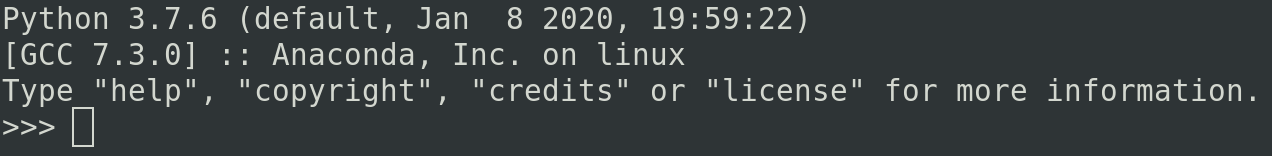
\includegraphics[width=8cm]{ressources/console.png}
                      \captionof{figure}{Console Python}
                      \label{console}
                  \end{center}
            \item Écrire les codes suivants puis valider. Observer les résultats obtenus.
                  \begin{center}
                      \begin{lstlisting}[language=Python , basicstyle=\ttfamily\small, xleftmargin=2em, xrightmargin=2em]
3+4
\end{lstlisting}
                      \begin{lstlisting}[language=Python , basicstyle=\ttfamily\small, xleftmargin=2em, xrightmargin=2em]
3<4
\end{lstlisting}
                  \end{center}
        \end{enumerate}
    \end{activite}


\end{frame}
\begin{frame}
    \frametitle{}
    Il peut rapidement être fastidieux d'écrire un programme dans la console Python. Un \textbf{Environnement de Développement Intégré} permettra d'écrire plusieurs lignes de code puis se chargera d'envoyer toutes ces lignes à l'interpréteur. De plus, il sera possible d'enregistrer le programme dans un fichier.

\end{frame}
\begin{frame}[fragile]
    \frametitle{}

    \begin{activite}
        \begin{enumerate}
            \item Dans l'espace personnel de l'ordinateur, créer un dossier \textbf{\texttt{NSI}}
            \item Ouvrir un EDI au choix: Spyder, Pyzo, EduPython.
            \item Écrire le programme suivant dans la partie gauche de l'EDI.
                  \begin{center}
                      \begin{lstlisting}[language=Python , basicstyle=\ttfamily\small, xleftmargin=2em, xrightmargin=2em]
print(3+4)
print(3<4)
\end{lstlisting}
                  \end{center}

        \end{enumerate}
    \end{activite}

\end{frame}
\begin{frame}
    \frametitle{}
    \setcounter{compteuractivite}{2}

    \begin{activite}
        \begin{enumerate}
            \setcounter{enumi}{3}
            \item Enregistrer le programme dans le dossier \emph{NSI} sous le nom \textbf{\texttt{premier.py}}
            \item Exécuter le programme en cliquant sur la flèche verte (figure \ref{execution}) ou en appuyant sur la touche \emph{F5}. Le code est exécuté dans la console en bas à droite.
                  \begin{center}
                      \centering
                      
\includegraphics[width=1cm]{ressources/execution.png}
                      \captionof{figure}{Exécuter le programme}
                      \label{execution}
                  \end{center}
        \end{enumerate}
    \end{activite}

\end{frame}
\subsection{Variables}
\begin{frame}
    \frametitle{Variables}

    En première approche, nous pouvons considérer une \textbf{variable} comme une boîte qui contient une information. Cette information peut être de plusieurs natures (nombre, texte, tableau...)
    \note{On ne s'occupe plus de l'adressage mémoire, du passage dans les registres.}
\end{frame}
\begin{frame}[fragile]
    \frametitle{}

    \begin{activite}
        \begin{enumerate}
            \item Dans le dossier \emph{NSI}, créer un fichier \textbf{\texttt{jeu\_de.py}}
            \item Écrire le code suivant:
                  \begin{lstlisting}[language=Python , basicstyle=\ttfamily\small, xleftmargin=2em, xrightmargin=2em]
de1 = 3
\end{lstlisting}
        \end{enumerate}

    \end{activite}


\end{frame}
\begin{frame}
    \frametitle{Correction}

    \begin{center}
        \begin{tikzpicture}
            \draw (0,1) -- (0,0) -- (1,0) -- (1,1);
            \node (3) at (3,2) {3};
            \node at (.5,-.2) {de1};
            \draw[->,>=latex] (3) to[bend right=40] (.5,.5);

        \end{tikzpicture}
        \captionof{figure}{Affectation}
    \end{center}

\end{frame}
\begin{frame}[fragile]
    \frametitle{}
    \begin{aretenir}[Remarque]
        Même si cela est possible en Python nous n'utiliserons pas de caractère accentué dans les noms de variables. De plus nous pourrons utiliser le signe \_ pour \emph{coller} plusieurs mots dans un nom.
        \begin{lstlisting}[language=Python , basicstyle=\ttfamily\small, xleftmargin=2em, xrightmargin=2em]
le_de = 3
\end{lstlisting}
    \end{aretenir}

\end{frame}
\begin{frame}[fragile]
    \frametitle{}


    \begin{aretenir}[Remarque]
        Le signe \textbf{=} n'est pas à comprendre au sens mathématique. C'est un signe d'affectation. Ainsi l'instruction
        \begin{lstlisting}[language=Python , basicstyle=\ttfamily\small, xleftmargin=2em, xrightmargin=2em]
3 = a
\end{lstlisting}
        est juste mathématiquement mais ne signifie rien en Python.
    \end{aretenir}

\end{frame}
\subsection{Entrée/Sortie}
\begin{frame}[fragile]
    \frametitle{Entrée/Sortie}

    L'instruction
    \begin{lstlisting}[language=Python , basicstyle=\ttfamily\small, xleftmargin=2em, xrightmargin=2em]
input()
\end{lstlisting}
    attend une valeur de l'utilisateur. Cependant, la valeur est inaccessible. Il faut donc la stocker dans une variable:
    \begin{lstlisting}[language=Python , basicstyle=\ttfamily\small, xleftmargin=1em, xrightmargin=1em]
proposition = input("Choisir une valeur du dé: ")
\end{lstlisting}


\end{frame}
\begin{frame}[fragile]
    \frametitle{}

    L'instruction
    \begin{lstlisting}[language=Python , basicstyle=\ttfamily\small, xleftmargin=2em, xrightmargin=2em]
print("mon texte")
\end{lstlisting}
    affiche \emph{mon texte} à l'écran. Il est possible d'afficher le contenu d'une variable:
    \begin{lstlisting}[language=Python , basicstyle=\ttfamily\small, xleftmargin=2em, xrightmargin=2em]
print(proposition)
\end{lstlisting}
    Il ne faut alors pas mettre de guillemets.

\end{frame}
\begin{frame}[fragile]
    \frametitle{}

    \begin{aretenir}[Remarque]
        La valeur récupérée par \textbf{\texttt{input}} est une chaîne de caractère. Il est nécessaire d’insérer l’appel \texttt{\textbf{input()}} dans une fonction \texttt{\textbf{int()}} pour convertir la réponse en un entier:
        \begin{lstlisting}[language=Python , basicstyle=\ttfamily\small, xleftmargin=1em, xrightmargin=1em]
proposition = int(input("Choisir: "))
\end{lstlisting}
    \end{aretenir}

\end{frame}
\subsection{Comparaison}
\begin{frame}[fragile]
    \frametitle{Comparaison}
    Pour vérifier la valeur du dé proposée par l'utilisateur, il faut la comparer avec celle du programme.

    \begin{aretenir}[]
        L'instruction
        \begin{lstlisting}[language=Python , basicstyle=\ttfamily\small, xleftmargin=1em, xrightmargin=1em]
a == b
\end{lstlisting}
        renvoie \textbf{\texttt{True}} si les variables \textbf{\texttt{a}} et \textbf{\texttt{b}} sont égales, \textbf{\texttt{False}} sinon. Il faut noter l'emploi du \textbf{\texttt{==}} pour ne pas confondre avec le signe d'affectation.
    \end{aretenir}


\end{frame}
\begin{frame}[fragile]
    \frametitle{}
    \begin{aretenir}[]
        Le mot-clé \textbf{\texttt{if}} évalue la comparaison qui le suit et agit en conséquence.
    \end{aretenir}
    \begin{center}
        \begin{lstlisting}[language=Python , basicstyle=\ttfamily\small, xleftmargin=2em, xrightmargin=2em]
if a == b:
    print("a et b sont égaux.")
else:
    print("a et b sont différents.")
\end{lstlisting}
        \captionof{code}{Comparaison (le \textbf{\texttt{else}} est facultatif).}
        \label{CODE}
    \end{center}

\end{frame}
\begin{frame}
    \frametitle{}

    \begin{activite}
        Compléter le programme \textbf{\texttt{jeu\_de}} pour que le message \textbf{gagné} s'affiche si la proposition de l'utilisateur est correcte, \textbf{perdu} sinon.
    \end{activite}

\end{frame}
\begin{frame}[fragile]
    \frametitle{Correction}

    \begin{center}
        \begin{lstlisting}[language=Python , basicstyle=\ttfamily\small, xleftmargin=2em, xrightmargin=2em]
if de1 == proposition:
    print("Gagné")
else:
    print("Perdu")
\end{lstlisting}
    \end{center}

\end{frame}
\subsection{Répétition}
\subsubsection{Boucle non bornée}
\begin{frame}
    \frametitle{Boucle non bornée}

    \begin{aretenir}[]
        Une boucle non bornée répète une instruction tant que la condition est vérifiée.
    \end{aretenir}

\end{frame}
\begin{frame}[fragile]
    \frametitle{}

    \begin{activite}
        \begin{enumerate}
            \item Dans un nouveau fichier tester le programme ci-après:
                  \begin{lstlisting}
compteur = 10
while compteur > 0:
    print(compteur)
    compteur = compteur - 1
print("Boum")
\end{lstlisting}
            \item En anglais, que signifie \textbf{\texttt{while}}?
            \item À quelle ligne compare-t-on le compteur avec la valeur limite?
            \item Quel est le rôle de la ligne 4? Que se passera-t-il si cette ligne est retirée?
        \end{enumerate}
    \end{activite}

\end{frame}
\begin{frame}
    \frametitle{Correction}

\begin{itemize}
    \item<1-> \textbf{Tant que} le contenu de la variable \textbf{\texttt{compteur}} est un entier supérieur à 10, les lignes 3 et 4 sont répétées.
    \item<2-> La ligne 5 n'est pas dans la boucle: elle n'est pas \emph{indentée}.
    \item<3-> Si la ligne 4 est retirée, la boucle tourne indéfiniment.
\end{itemize}

\end{frame}
\begin{frame}
    \frametitle{}

    \begin{activite}
\begin{enumerate}
    \item Modifier le programme \textbf{\texttt{jeu\_de}} pour qu'il interroge l'utilisateur tant que ce dernier ne donne pas la bonne réponse.
    \item Ajouter un \textbf{\texttt{compteur}} qui compte le nombre de tentatives.
\end{enumerate}
    \end{activite}

\end{frame}
\begin{frame}[fragile]
    \frametitle{Correction}

\begin{center}
\begin{lstlisting}[language=Python , basicstyle=\ttfamily\small, xleftmargin=2em, xrightmargin=2em]
de1 = 3
proposition = 0
while de1 != proposition:
    proposition = int(input("Choisir: "))
\end{lstlisting}
\end{center}

\end{frame}
\begin{frame}[fragile]
    \frametitle{Correction}

\begin{center}
\begin{lstlisting}[language=Python , basicstyle=\ttfamily\small, xleftmargin=2em, xrightmargin=2em]
de1 = 3
proposition = 0
compteur = 0
while de1 != proposition:
    compteur = compteur + 1
    proposition = int(input("Choisir: "))
print(compteur)
\end{lstlisting}
\end{center}

\end{frame}
\subsubsection{Boucle bornée}
\begin{frame}[fragile]
    \frametitle{Boucle bornée}

    \begin{activite}
    \begin{enumerate}
    \item Tester le programme ci-après:
    \begin{lstlisting}[language=Python , basicstyle=\ttfamily\small, xleftmargin=1em, xrightmargin=1em]
for compteur in range(10):
    print(compteur)
\end{lstlisting}
    \item Lire la documentation de la fonction \emph{range}:
    \begin{center}
    \url{https://tinyurl.com/rangepython}
    \end{center}
    \item Adapter le code précédent pour afficher:
    \begin{itemize}
    \item 6
    \item 7
    \item 8
    \end{itemize}
    \item Adapter le code précédent pour afficher:
    \begin{itemize}
    \item 0
    \item 3
    \item 6
    \item 9
    \end{itemize}
\end{enumerate}
\end{activite}
\end{frame}
\begin{frame}[fragile]
    \frametitle{Correction}

\begin{center}
\begin{lstlisting}[language=Python , basicstyle=\ttfamily\small, xleftmargin=2em, xrightmargin=2em]
for compteur in range(6,9):
    print(compteur)
\end{lstlisting}
\captionof{code}{Borne de départ}
\end{center}   
\begin{center}
\begin{lstlisting}[language=Python , basicstyle=\ttfamily\small, xleftmargin=2em, xrightmargin=2em]
for compteur in range(0,10,3):
    print(compteur)
\end{lstlisting}
\captionof{code}{Pas}
\end{center}
\end{frame}
\subsection{Bibliothèque}
\begin{frame}
    \frametitle{Bibliothèque}

    Le jeu de dés semblerait être plus intéressant si la réponse n'était pas \emph{codée en dur} dans le programme.

\end{frame}
\begin{frame}[fragile]
    \frametitle{}
\note{Première approche rapide des bibliothèques}
Python fournit des \textbf{bibliothèques} spécialisées. La bibliothèque \textbf{\texttt{random}} permet de générer des nombres aléatoires.
\begin{center}
\begin{lstlisting}[language=Python , basicstyle=\ttfamily\small, xleftmargin=2em, xrightmargin=2em]
from random import randint

de1 = randint(1,6)
\end{lstlisting}
\captionof{code}{Générer un entier aléatoire}
\label{aleatoire}
\end{center}
\begin{activite}
Modifier le programme \textbf{\texttt{jeu\_de}} en utilisant le code \ref{aleatoire}.
\end{activite}
\end{frame}
\end{document}
